%%% Important. To have correct table numberings
\renewcommand{\thetable}{\thesection\alph{table}}

\chapter[Excellence]{Excellence}
\label{cha:excellence}
\instructions{
Your proposal must address a work programme topic for this call for proposals. \\
\textit{This section of your proposal will be assessed only to the extent that it is relevant to that topic.}\\
}

\section{Objectives}
\label{sec:objectives}
\instructions{
Describe the overall and specific objectives for the project1, which should be clear, measurable,
realistic and achievable within the duration of the project. Objectives should be consistent with
the expected exploitation and impact of the project (see section 2).
}

The objective of this proposal is to build a detailed selection function for the astrophysical data collected during the survey of the sky carried out by the European Space Agency's Gaia Mission. The selection function will be provided to the scientific community in the form of numerical tables and source code that allow users to apply the selection function to their scientific analyses. The outcome will be a dramatic boosting of the scientific exploitation of the Gaia mission data; the unlocking of science applications based on Gaia data that are not possible now; and an increase in scientific publications from this flagship European space mission. In detail the objectives are:

\begin{enumerate}
    \item Develop a detailed mathematical formulation of a survey selection function, where the goal is to keep this as general as possible even if in this project the focus is on the Gaia survey. This will ensure that the expertise built up in this project is transferable to other astronomical surveys. The mathematical formulation should account for the layering of user imposed sample selections on top of the survey selection function and allow for a description of the selection function of combinations of surveys.
    \item Research and develop a detailed description and modelling of the Gaia survey selection function and do the same for the combination of Gaia and other surveys. The results will set the requirements for the next two items.
    \item Provide a detailed practical implementation of the Gaia selection function in the form of auxiliary data, which will be accessible through the ESA Science Data Centre, and open source tools, which will be made available through code hosting websites. 
    \item Develop tools to incorporate the selection function in scientific analyses. These tools should allow for combining the Gaia survey selection function with user imposed sample restrictions and for combining Gaia with other surveys. The tools will be made available as open source code through code hosting websites.
    \item Apply the selection function tools to example science cases. This will serve to demonstrate the benefits of carefully accounting for the selection function and at the same time provide worked examples to the community of prospective users of these tools.
\end{enumerate}

The long term curation of the results from this project will be ensured through the availability of the auxiliary data through the ESA Gaia archive and by source code for the uers tools being embedded in or affiliated to the Astropy project.

\subsection{Boosting the science exploitation of Gaia data}
\label{sec:needforselectionfunction}

The European Space Agency's Gaia Mission \cite{2016A&A...595A...1G} is the most successful of ESA's space astronomy missions as measured by the publication rate of papers using its data in one form or another. Over 2500 papers appeared between April 2018 and February 2020 that use data from the second Gaia data release\footnote{As indicated by the number of  \href{https://ui.adsabs.harvard.edu/search/q=citations(bibcode\%3A2018A\%26A...616A...1G)&sort=date\%20desc\%2C\%20bibcode\%20desc&p_=0}{citations to the Gaia DR2 release paper}}. Among the many high profile science results published by European groups are the discovery of a spiral in the phase space structure of the Milky Way's disk (\cite{2018Natur.561..360A}, indicative of a recent disturbance, most likely due to the Sagittarius dwarf galaxy), the first direct observational evidence of crystallization in the interiors of white dwarfs (\cite{2019Natur.565..202T}, confirming a fifty year old prediction), and the uncovering of a major event 10 billion years into the Milky Way's past when a collision with a dwarf galaxy took place which contributed to the build-up of the Milky Way's stellar halo and thick disk \cite{2018Natur.563...85H, 2018MNRAS.478..611B, 2019arXiv190904679B}. 

But while there are numerous exciting results that are starting to transform many different fields of astrophysics, most of these have focused on `low hanging fruit' in the Gaia data archive, and have barely scratched the surface of the information contained in the Gaia data. Specifically, almost all analyses to date have exploited the astounding Gaia data precision and accuracy on individual objects, but have side-stepped performing or exploiting \textbf{population studies}, i.e. the \textsl{statistical distribution of objects with certain properties}. For example, a result as elementary as a good determination of the radial profile of the Milky Way's disk stars --- by simply counting them as a function of position --- has yet to be carried out. This is because such studies inevitably require knowledge of the \textbf{selection function}, i.e. the probability that an object of certain physical properties at a certain position in space would be catalogued by Gaia. This knowledge is indispensable for any population study of objects; and population studies are the very core of the Gaia mission, with its billions-of-objects catalogue.

In practice the community so far has often resorted to drastic cuts, on object properties and Gaia data quality flags, to arrive at samples whose selection function is very simple (avoiding for example the well known problems associated with the estimation of distance as the inverse of the parallax \cite{2018A&A...616A...9L}). Yet, such analyses grossly under-exploit the information content of the Gaia data set, often by orders of magnitude.

Consequently, many high-profile science cases for which Gaia was built cannot be realized as long as the selection function of the Gaia survey is not known well, currently neither to the Gaia DPAC team, nor to the community. It is the single goal of this proposal to remedy this shortcoming and dramatically boost (yes, yet further!) the astrophysical utility of the Gaia mission, by comprehensively characterizing the catalog's selection function.

The Gaia selection function results from a highly non-trivial combination of the on-board source selection, telemetry losses, selections on data quality during processing, the scanning pattern of the mission, and selections on quality before the publication of the processed data in the Gaia archive. As a result, the selection function for Gaia has only been characterized in highly simplified ways \memo{(provide literature references in the motivation section below)} even though it will be crucial for a full exploitation of the intrinsic science potential of the Gaia data, in particular also in view of the legacy value of the Gaia archive which will remain the standard in fundamental astrophysical data for decades to come.

\subsection{Context}
\label{sec:context}

ESA's Gaia mission \cite{2016A&A...595A...1G} represents a European breakthrough in astrophysics, a cornerstone mission which was launched in 2013 aimed at producing the most accurate 3D map of the Milky Way to date. The resulting stereoscopic census of our Galaxy represents a giant leap in astrometric accuracy (reaching the 10--20 micro-arcsecond regime, which is equivalent to knowing the 3D positions of stars to 10 per cent precision over distances as large as $20\,000$ to $30\,000$ light-years) complemented by the only full sky homogeneous photometric survey with an angular resolution comparable to that of the Hubble Space Telescope, as well as the largest spectroscopic survey ever undertaken. 

The primary scientific aim of the mission is to map the structure of our Galaxy and unravel its formation history and subsequent evolution. Current cosmological models envisage the formation of large galaxies through the merging of smaller structures. Deciphering the assembly history of our Galaxy requires a detailed mapping of the structure, dynamics, chemical composition, and age distribution of its stellar populations. Ideally one would like to `tag' individual stars to each of the progenitor building blocks of the Galaxy \cite{2002ARA&A..40..487F}. The Gaia mission is designed to provide the required fundamental data in the form of distances (through parallaxes), space velocities (through proper motions and radial velocities) and astrophysical characterisation (through multi-colour photometry) for massive numbers of stars throughout most of the Galaxy. It should be stressed however that Gaia is not simply a `Milky Way mission' but is truly a multi-faceted {\em astrophysics mission} which will provide exciting scientific results covering many topics including: fundamental stellar physics across the Hertzsprung-Russell diagram, the characterisation of tens of millions of binary stars, unique samples of variable stars of nearly all types (including key cosmological distance calibrators), detection and orbital classification of thousands of exo-planetary systems, a comprehensive survey of objects ranging from huge numbers of minor bodies in our Solar System, through galaxies in the nearby Universe, to over a million distant quasars. Gaia will also provide a number of stringent tests of general relativity. Last but not least, a massive survey such as Gaia will uncover many surprises that the Universe still holds in store for us.

The data processing for the Gaia mission is carried out by a European consortium of institutes and funding agencies, the Data Processing and Analysis Consortium (DPAC). The task of the DPAC is to turn the raw telemetry from Gaia into data products ready for use by astronomers and scientists around the world. The data products are both the basic astrometric, photometric, and spectroscopic results as well as advanced data products, such as the astrophysical characterization of stars, derived from the former. Through an independent unit within the consortium the DPAC also ensures the quality of the published data through extensive technical and scientific validation. The publicly released data, which are disseminated through the ESA Science Data Center and its partners, are accompanied by extensive documentation which is also produced by DPAC. It should be stressed here that the DPAC holds no proprietary rights to the data which means that once the data products are validated and documented they are released publicly and world-wide without delay. In this sense Gaia represents a uniquely open survey concept.

From the early days of the Gaia mission it was foreseen to have incremental data releases based on increasing amounts of collected telemetry. The various data products would be released in stages (where, for example, some of the advanced data products such as exoplanet catalogues can only be released after sufficient data has been collected and the various astrometric calibrations have reached the required levels of precision) and with increasing accuracy for each release. To date two data releases have taken place, Gaia DR1 in September 2016 and Gaia DR2 in April 2018. Both releases have been highly successful and have had major impacts on the fields of Galactic archaeology; Milky Way mass estimation; stellar streams, dwarf galaxies, globular clusters; open clusters; white dwarfs; the characterization of exoplanet host stars and determining the absolute sizes of protoplanetary disks, to name a number of prominent examples. The studies of individual stars and stellar systems benefit immensely from the now easily available high precision parallax data.

The next releases foreseen are Gaia EDR3 in the third quarter of 2020 and Gaia DR3 in the second half of 2021. The following release (Gaia DR4) will be based on all data collected during the nominal mission lifetime of Gaia and feature the full suite of data products, including the epoch data (individual measurements) for the astrometry, photometry, and spectroscopy\footnote{See the \href{https://www.cosmos.esa.int/web/gaia/release}{Gaia data release scenario} pages.}. These future Gaia data releases are expected to have an even larger impact on astronomy due to the much richer set of data products allowing for the combination of high accuracy astrometry and radial velocities with detailed astrophysical characterization of the source in the Gaia catalogue (stellar parameters including chemical compositions and variability, parameters of multiple stars and exoplanets, medium resolution spectra around the Ca triplet region for millions of stars to magnitude 13, low resolution prism spectrophotometry for all sources in the Gaia catalogue). 

Despite the major successes of Gaia DR1 and Gaia DR2 there is one serious weakness of the releases: the DPAC does not provide a detailed selection function for the Gaia survey. This aspect has never been included in the funded DPAC efforts and will not be added as DPAC work in the future. This implies that major Gaia science cases cannot be addressed by the astronomical community to the full potential of the quality of the data. In \secref{sec:scientific-motivation} we motivate why a detailed selection function is needed and how this will enhance the scientific exploitation of the data from this flagship European space mission. 

\paragraph{Gaia instruments and survey strategy} For the understanding of the work proposed here it is useful to briefly summarize the characteristics of the Gaia mission and how the measurements are collected and subsequently processed on ground. Much more detail can be found in the paper describing the Gaia mission \cite{2016A&A...595A...1G}. The Gaia spacecraft and its instruments were designed to collect data that will allow the determination of highly accurate positions, parallaxes, and proper motions for $>1$ billion sources brighter than magnitude $20.7$ in its white-light photometric band $G$ (covering the range $330$--$1050$~nm). The astrometry is complemented by multi-colour photometry, measured for all sources observed by Gaia, and radial velocities which are collected for stars brighter than $G\approx17$. Gaia carries two telescopes of which the collected light is combined into a single focal plane servicing the three main instruments. The astrometric instrument collects source images in the $G$-band, where the fundamental inputs to the astrometric data processing consist of the precise times when the image centroids pass a fiducial line in the focal plane of the instrument. The photometric instrument is realised through two prisms dispersing the light entering the field of view of two dedicated sets of CCDs. The Blue Photometer (BP) operates over the wavelength range $330$--$680$ nm, while the Red Photometer (RP) covers the wavelength range $640$--$1050$ nm. The data collected by the photometric instrument consists of low resolution spectrophotometric measurements of the source spectral energy distributions. The spectroscopic instrument, also called the radial-velocity spectrometer (RVS), collects medium resolution ($R\sim11\,700$) spectra over the wavelength range $845$--$872$~nm, centred on the Calcium triplet region. The spectra are collected for all sources to $G\approx17$ (16$^\text{th}$ magnitude in the RVS filter band).

The Gaia sky survey strategy is derived from that of the Hipparcos mission and and relies on the spacecraft slowly spinning around the axis perpendicular to the lines of sight of the two telescopes (which are separated by $106.5^\circ$. Every six hours the Gaia telescopes can scan a great circle on the sky with an across scan field of view size of $0.7^\circ$. By slowly precessing the spin axis around the direction to the Sun the full sky can be surveyed with optimal sky coverage uniformity over the five years nominal mission lifetime. 

The processing of the observations collected by Gaia is carried out by the DPAC through a series of complex pipelines which are part of a large iterative system (see section 7 in \cite{2016A&A...595A...1G}).

Although the Gaia survey selection function is seemingly very simple, with only a magnitude limit imposed on the observations (see \figref{fig:gsf_ideal}), each of the above components of the Gaia mission adds complexity to the survey selection function as illustrated in \figref{fig:gsf_realistic}. A few examples are listed here:
\begin{itemize}
    \item The data collection on the spacecraft is limited by the amount of sources that can be handled at any on time, meaning that for dense regions on the sky (above $10^6$, $750\,000$, and $35\,000$ sources~deg$^{-2}$ for the astrometric, photometric, and spectroscopic instruments respectively) not all sources can be measured, leading to brighter effective survey limits in those regions. In addition the on-board storage capacity limitations combined with available ground station time lead to deletion of data on occasions when both Gaia telescopes are scanning along the Galactic plane for prolonged periods of time.
    \item Despite the optimal sky survey strategy realized through the revolving scanning technique, the number of times any given source is observed does vary with celestial position, in particular with the ecliptic latitude.
    \item Decisions are made along each of the various on-ground data processing steps on which data and/or sources to process, where periods of ``bad inputs'' are excluded. This leads to gaps in the time coverage of measurements for a given source or to effectively brighter survey limits covering certain time periods (which translates to certain areas on the sky). Additionally, in early data releases the processing for certain data products may be limited to brighter sources or sources with specific astrophysical characteristics.
\end{itemize}
Each of the above examples complicates the Gaia survey selection function which in the end is very non-trivial to describe and handle. Nevertheless we must make an effort to provide the best possible description of the selection function as well as tools to incorporate it into scientific analyses as we motivate in \secref{sec:scientific-motivation}.

\paragraph{Timing of this proposal} We stress here that the time to research a detailed selection function for the Gaia survey is \emph{now}:
\begin{itemize}
    \item To understand the selection function in detail, accounting for all the issues described above and in \secref{sec:concept}, requires access to the Gaia spacecraft and data processing expertise within DPAC and ESA. It is thus essential to start this work while the DPAC is still active.
    \item Already now the availability of a selection function for the Gaia DR2 catalogue would represent a major boost to the science exploitation of those data.
    \item Which each upcoming Gaia data release the complexities of the selection function will increase thus making any effort postponed to the future much more costly in terms of human resources required.
\end{itemize}

\subsection{Scientific motivation}
\label{sec:scientific-motivation}

\subsubsection{The selection function: definition and indispensability}

For any `statistical' study using a catalog, for any study where it matters quantitatively how common or rare a certain type of object or circumstance is, the selection function of a catalog is arguably as important as the catalog itself. The catalog \textit{selection function}, $S_C(y)$, is a function of the observable (and thereby underlying physical) properties, $y$, of any astronomical objects; and it specifies the probability that an object of properties $y$ will enter the (Gaia) catalog. A generic and central way of learning from any catalog, is to envision a set of physical or mathematical models $\lambda_0(z\given\theta)$ -- that predicts the
distribution of true quantities $z$, given a set of model parameters $\theta$ -- and then ask
what the `data' (the catalog entries) $\lambda_C(y\given\theta)$ tell us about the relative plausibility. 
The relation between these quantities is generically
\begin{equation}
\lambda_C(y\given\theta) = S_C(y)\,\int p(y\given z)\,\lambda_0(z\given\theta)\,{\textrm{d}} z = S_C(y)\,\lambda_0(y\given\theta),
\label{eqn:selfunc_definition}
\end{equation}
where $z$ is the vector of true values (\emph{vs.} the observed values $y$). 
\textbf{This immediately shows that no inference, is possible without knowledge of $\mathbf{S_C(y)}$}. Most commonly the quantities $y_s$ on which the selection function really depends is only a modest subset of all the catalog entries, or all the quantities that are being modelled, $y$, the selection function separates $S_C(y_s) \times S_0(y_{other})$, with $S_0(y_{other})\approx 1$. 
For the Gaia catalog selection function, the quantities $y_s$ are (in presumably good approximation): the sky position $(\alpha,\,\delta)$ of an object, its magnitude in the visible G band, and its BP$-$RP color from the spectrophotometric bands.\footnote{For objects with very high proper motions, e.g. in the Solar system, the selection function may also depend on $\vec{\mu}$; this interesting regime, affecting a very small fraction of the Gaia detections, is not the focus of this proposal.} These four quantities are a small subset of the Gaia catalog entries. So, why is it hard to determine a good approximation of the Gaia catalog selection function, $S_C(y_s)$? This is because 
$S_C(y_s)$ is such a complex function of the $y_s$: the sky position enters through the source density (``crowding'') and the scanning pattern, which sets the number of observation epochs and the distribution of roll angles; the roll angle in turn determines the (sky) direction in which the BP, RP and RVS spectra are dispersed, which in turn determines the probability that they are rendered unusable dues to source-source contamination. The magnitudes determine not only the obvious aspect of the photon noise, but -- in conjunction with the source density -- also the decision of parsing the data into postage stamps for processing. This will be detailed in the methodology section of this proposal.

Given that $S_C(y_s)$ has not (yet) been determined for Gaia, why is it that many %results of
widely accepted results have already come from analysing the distribution of Gaia catalog entries for large samples? This is for a number of reasons. First, some studies have essentially ignored (at their own peril) the selection function, thereby implicitly assuming $S_C(y_s)\approx 1$ for the regime of interest. The second and most frequent regime so far is that one can make additional ``sample cuts'' by defining
\begin{equation*}
    S_{cut}(y) = \begin{cases} 1 &\mbox{if\ \ } y \mbox{\ \ within cuts} \\ 
0 &\mbox{\ \ else} \end{cases}
\end{equation*}
If one then models only the restricted data $\lambda_{cut}(y\given\theta)$, Eq.\ref{eqn:selfunc_definition} becomes simple, as one the can sensibly adopt
%as the right hand side can be supposedly approximated as 
\begin{equation*}
    \lambda_{cut}(y\given\theta) \approx S_C(y) \times S_{cut}(y)\, \lambda_0(y\given \theta) \approx  \begin{cases}  \lambda_0(y\given \theta) &\mbox{if\ \ } y \mbox{\ \ within cuts} \\ 
0 &\mbox{\ \ else.} \end{cases}
\end{equation*}
A pertinent example would be that for a 'stellar halo study' $S_{cut}(y)$ limits the analysis to, say, blue-ish (BP$\_$RP$<1$) stars of $13.5<G<17.5$ at high Galactic latitudes, away from Globular clusters and the Magellanic Clouds. Then the assumption that the small sub-sample is nearly complete within the stated $S_{cut}(y)$  is defensible.
%}

The third regime is that one can analyze the distribution of quantities in $p(y_{other})$, or $p(y_{other}~|~y_s)$: the most obvious case is to analyze the 3D kinematic in the Solar neighbourhood. The fourth regime is of course, that the selection function $S_C(y_s)$ has been ``properly'' determined and included in the modelling [REF]; however this has only happened to date for very small sub-regimes of the space spanned by $y_s$ in the Gaia catalog.


\textbf{It is the comprehensive construction of this (approximate) selection function, $S_C(y_s)$, that is at the heart of this proposal.} As we now sketch with a few examples, without its robust and precise knowledge it is impossible to extrapolate from \textit{statements about the objects' population in a catalog} into \textit{insights in fundamental physics and astrophysics}.

\subsubsection{Highlight Gaia Science that cannot be done without a Good Selection-Function}
We now proceed to highlight a few science cases central to Gaia's scientific success that absolutely require a well-determined selection function to be feasible\footnote{By `feasible' in this context we mean: able to address a science question with a quantitative understanding of the dominant source of systematic uncertainty; and not falling short by more than an order-of-magnitude of the full pertinent information content of the Gaia catalog.}.
To illustrate the kinds of selection effects that can occur in the Gaia data we refer to figures \ref{fig:6dsample}--\ref{fig:bulge}. These figures serve also to reinforce the points made in the following text.
\\

\begin{figure}
    \centering
    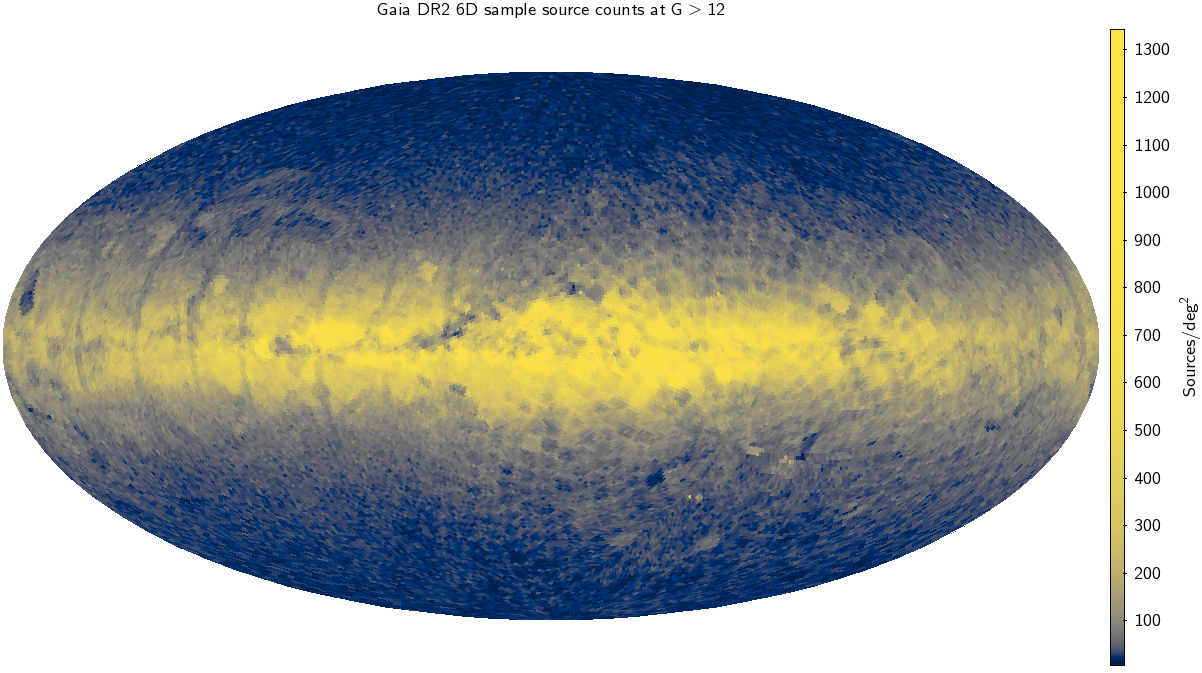
\includegraphics[width=\linewidth]{DR2_6DSample_Source_Counts_Ggt12.png}
    \caption{Source density distribution on the sky (no.\ per square degree) of stars in the Gaia DR2 catalogue for which a radial velocity is listed and which are fainter than $G=12$. The sky projection is in Galactic coordinates with the Milky Way bulge in the centre of the image and the longitude increasing to the left. Note the prominent patterns of squares in the southern hemisphere on the lower right hand side of the figure. These are imprints of photographic plates on which the Guide Star Catalogue is based which was one of the surveys used to construct the Initial Gaia Source List \cite{2014A&A...570A..87S}. This list was used to bootstrap the creation of the Gaia source list (see \secref{sec:methods}). Imprints from the Sloan Digital Sky Survey spectroscopic survey can be seen as dark stripes crossing the Galactic plane on the left hand side. Although these imprints will gradually disappear in future Gaia data releases, this figure is a good illustration of the complications that can arise for selection functions of combined surveys.}
    \label{fig:6dsample}
\end{figure}

\begin{figure}
    \centering
    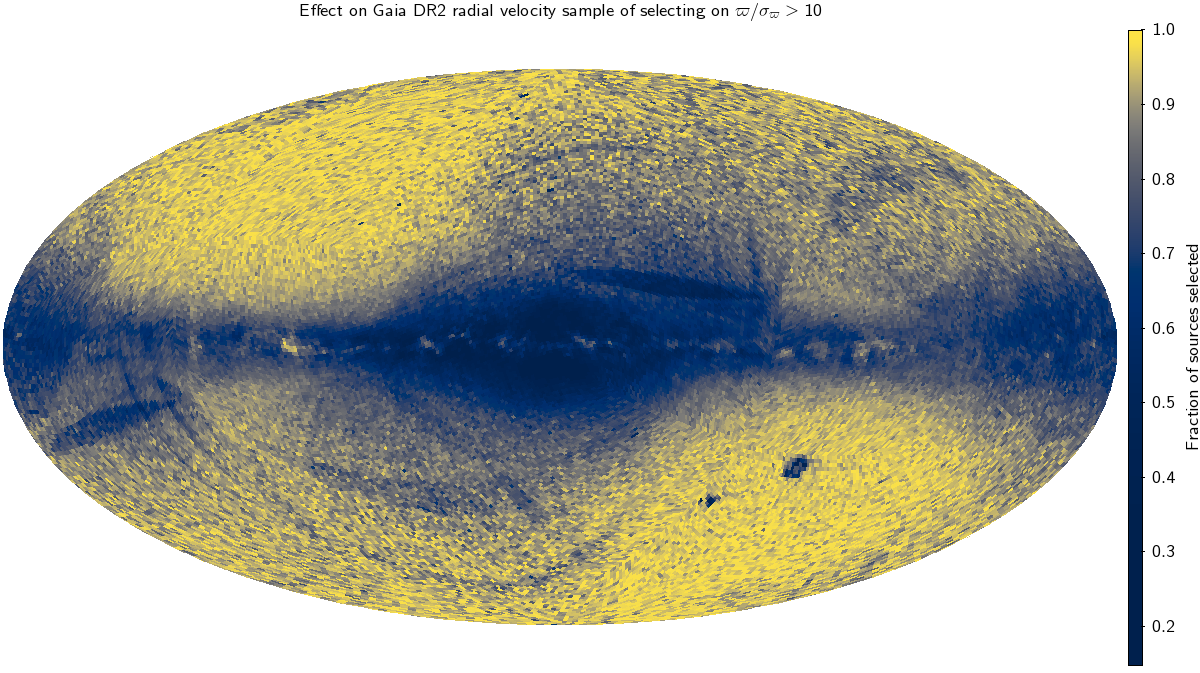
\includegraphics[width=\linewidth]{SelectionEffect6DSamplePlxSnrGt10.png}
    \caption{The fraction of stars selected from the Gaia DR2 sample for which radial velocities are listed, when demanding that the parallax is larger than 10 times its uncertainty. Note how the ecliptic pole regions on the top left and bottom right are strongly favoured, whereas the fraction of selected source drops dramatically along the Galactic plane. In addition there are oddly shaped regions with a lower fraction of selected sources. These reflect a combination of the scanning strategy followed by Gaia and filtering on data quality at various stages in the data processing.}
    \label{fig:6dplxsnrgt10}
\end{figure}
\noindent\textbf{A) 3D-Mapping of the Milky Way}

\begin{figure}
    \centering
    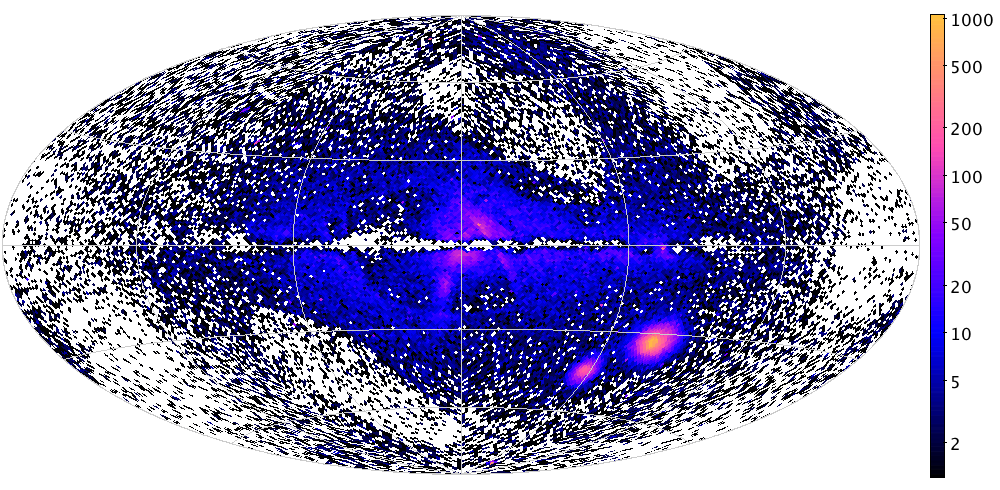
\includegraphics[width=0.7\linewidth]{DR2_skyPlot_sos_RRL_inv.png}
    \caption{The sky distribution of confirmed RR Lyrae variables in the Gaia DR2 catalogue. Note the very strong selection effects on the sky due to the combination of the scanning strategy, the constraints on the minimum number of observations for classifying variable stars, and data quality filtering in the processing pipelines. For details see \cite{2018A&A...618A..30H}.}
    \label{fig:rrl}
\end{figure}

\begin{figure}
    \centering
    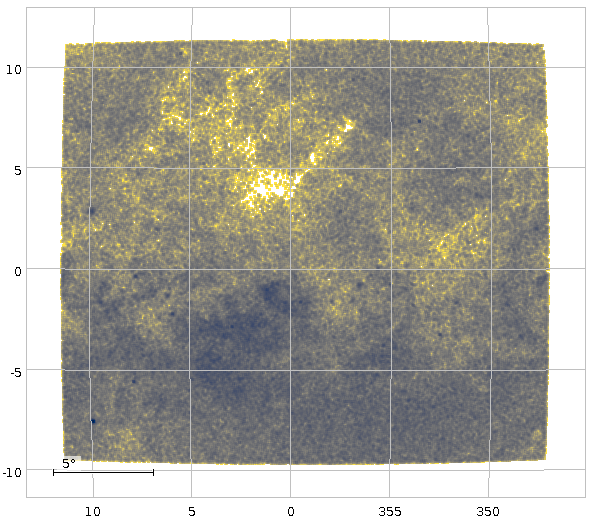
\includegraphics[width=0.5\linewidth]{img/BulgeRegionGlt13.png}\hfil
    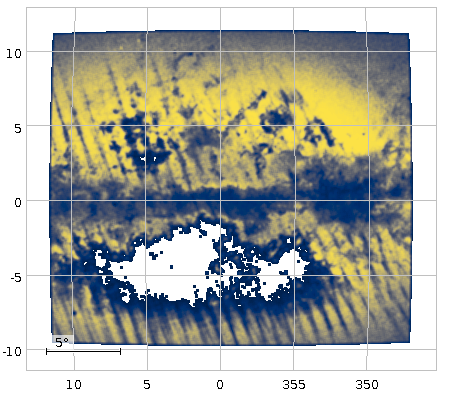
\includegraphics[width=0.5\linewidth]{img/BulgeRegionG20p65to20p70.png}
    \caption{\textbf{Left} The distribution on the sky of sources brighter than $G=13$ (300 thousand sources) in the direction of the Milky Way bulge region. No obvious selection effects are apparent, the darker regions being due to clouds of dust blocking the light from the stars behind them. The white pixels are empty of sources due to severe dust effects.\textbf{Right} The same for sources with $20.65<G<20.70$ (4 million sources). Note the strong striping pattern which again reflects the combination of the Gaia sky scanning strategy and the filtering on data quality during the data processing. The white areas are due to a combination of dust effects and the drop in catalogue completeness at these faint magnitudes.}
    \label{fig:bulge}
\end{figure}

Creating an unprecedented, large-scale 3D map of our Galaxy is arguably the central seminal goal of the Gaia mission, at the heart of setting the fundamental parallax precision science requirements. Yet, to date, no large-scale map of the stellar density (most of which is in the Galactic disk) has emerged. This is because 
such a density map is not merely the combination of the (catalogued) stars distribution $\{y_s\}$, in position, magnitude and color with distances, e.g. from parallaxes. Linking $\{y_s\}$ to $\rho_*(X,Y,Z)$ requires modelling the 3D dust distribution (there are large, coherent efforts underway to do this) and of $S_C(y_s)$. The selection function is so central here, as the quantities to be modelled, are exactly the quantities $y_s$ on which the selection depends!
\\

\noindent\textbf{B) Milky Way Dynamics and Distribution of (Dark) Matter}

Inferring the (dark) mass distribution, or the gravitational potential, in and around our Galaxy from modelling the 6D phase-space distribution of stars is another seminal and central science case for the overall Gaia mission. There are many sophisticated approaches to 'dynamical modelling', but the indispensable role of a well-understood selection function of the stars that serve as kinematic tracers can be illustrated with the arguably simplest form of dynamical modelling, the Jeans Equation. Consider the disk dynamics in the vertical direction (the `Oort limit'):
\begin{equation}
    \frac{\partial[\rho_*(R,z) \overline{v_z^2}(R,z)]}{\partial z}~+~\frac{1}{R}
    \frac{\partial[R \rho_* \overline{v_z v_R}]}{\partial R} + \rho_*\frac{\Phi(R,z)}{\partial z}=0 \mathrm{\ or\ \ } \frac{\partial[\rho_*(R,z) \overline{v_z^2(R,z)}]}{\partial z} + \rho_*\frac{\Phi(R,z)}{\partial z}=0,
    \label{eqn:Jeans}
\end{equation}
where the second form is for separable motions. Dynamics involves not only motions (e.g. dispersion), but also the tracer densities, and the spatial derivatives of the densities and motions. And the prediction of observables (the catalog entries) from $\rho_*(R,z)$ is of course linearly dependent on the selection function, and
on the spatial gradient of the selection function. \textbf{Therefore, Gaia data have taught us very little to date about dark matter near the Sun, whether the dark matter in the Milky Way has a cusp or a core}.

This is also why all initial high-profile analyses of the motions in Gaia data 
\citep{Katz2018a,Antoja2018a} were only \emph{kinematic} not \emph{dynamical} analysis. Traditionally, `rotation curve' has been the regime where the spatial tracer distribution matters least. But even the best Gaia rotation curve analyses \citep[e.g.][]{Eilers2019a} are limited in measuring exactly where dark matter starts to dominate the mass distribution in our Galaxy by the `asymmetric drift' 
the analogous radial terms to Eq.\,\ref{eqn:Jeans} including spatial tracer derivatives. Here, it is not only Gaia's selection function that needs to be known, but also that of the APOGEE survey; this present proposal also addresses the determination of survey-combined selection functions.\\

\noindent\textbf{C) Stellar Streams and `empty' dark matter halos with Gaia\ }

Dynamical analyses, where it is sensible to model $p(\vec{v}~|~\vec{x})$ rather than $p(\vec{v},\vec{x})$, depend less on detailed knowledge of the selection function, as $S_C(y)$ depends most strongly on $\vec{x}$, or on ($\alpha,\delta,D$). A beautiful recent example of this is \citet{Erkal2019}, which used Gaia proper motions (and other information) along the known `Orphan stream' to constrain the mass of the Magellanic Cloud. 
However, one needs not look further than the current holy grail of stellar stream science: the diagnosis of the impact of purported `empty' (i.e. star-free) dark matter sub-halos in the Milky Way: a close passage by of such a dark matter halos would create a gap or caustic in the stream. In the analysis of \citet{Bonaca2019} that provides the currently best evidence that such empty halos actually exist -- a central and untested prediction of $\lambda$CDM cosmogony -- the detailed knowledge of the selection function is the limiting systematic. 
\\

\noindent\textbf{D) Stellar Physics: Binary Stars in Gaia}

Among the many aspects of stellar physics where Gaia can be transformative, binary stars are an area of exceptional future importance \citep[e.g.][]{Breivik2019}. For example, Gaia has offered breakthroughs in identifying wide binaries, as adjacent stars of the same proper motion. Yet, this science direction brings up - and is severely limited by - another aspect of the selection function: the probability of getting selected is not only a function of its own properties, $y_s$, but also of its `neighbours'. This is illustrated in figure~\ref{fig:binaries}, which shows that the minimal distance $\Delta\theta$ at which a second (fainter) star has to be to also have a good proper motions measurement depends on the magnitude difference $\Delta G$. In \citet{ElBadry2019} this has been modelled well, but of course this modelling is only a small sub-aspect of a much broader selection function aspect.

\begin{figure}[ht!]
    \centering
    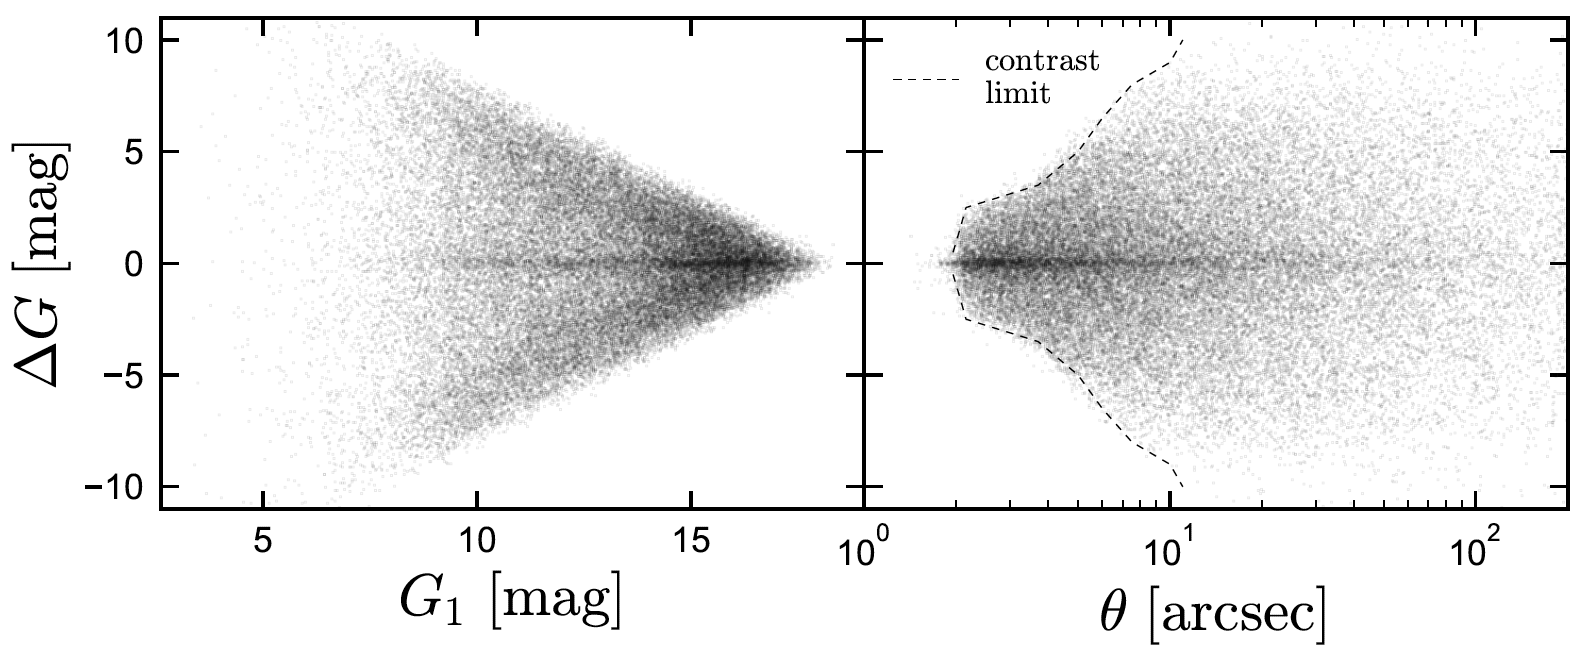
\includegraphics[width=0.7\linewidth]{img/BinarySelection_ElBadry.png}
    \caption{Illustration of the inherent complexities of the Gaia selection function (`contrast limit', right panel), when considering close pairs of sources, from \citet{ElBadry2019}, who discovered a population of twin-binaries (near-identical stars) to $\gtrsim 1000$~AU of unknown formation mechanism.
    Unsurprisingly, the minimal angular separation at which stars of a certain magnitude difference $\delta$G have both good proper motions (to be recognized as comoving) depends strongly on $\delta$G}
    \label{fig:binaries}
\end{figure}

Binaries are in this respect only the minimal case of either a star cluster or of crowded stellar fields in general. It is unsurprising that not a single publication using Gaia DR2 has appeared on one of the most interesting directions in our Galaxy, Baade's window.
In crowded field, often the catalog existence BP and RP ``magnitudes'',
which come from re-integrated slitless spectra, have a very complex dependence on position and magnitude.

\textbf{Without rigorous knowledge of $S_C(y_s)$ in the `crowded source' regime, binary science, cluster science and the central Galaxy will remain inaccessible to Gaia studies that do justice to the data's information content.}

There are added levels of complexity of determining and characterizing the selection function. Often, is of interest -- or at least tempting -- to make an extensive set of of quality flags part of a sample selection. If such cuts only eliminate a tiny subset, for reasons unrelated to the object's physical properties, this is without consequence. But if far-reaching cuts are made in quality flags such as RUWE (renormalized unit weight error) or on data uncertainties (velocity errors, fractional parallax errors) a whole new level of complexities arises. While in general it may be advisable to base sample selection on observables, not their uncertainties, the issue cannot be ignored. 
This is an area, where it may not be possible to devise (in the context of this proposal) a user-ready recipe for $S_C(y_s)$.

\textbf{Taken together, far better knowledge of the Gaia catalog selection function $S_C(y_s)$ is needed to
\begin{itemize}
    \item map our galaxy in 3D 
    \item do galaxy dynamics, constrain the distribution of dark matter and detect `empty' dark matter halos
    \item  unleash Gaia's potential for stellar astrophysics, even on aspects as elementary as estimating luminosity functions and frequencies of special objects, or learn about binary stars.
    \item start exploring what Gaia can teach us in `crowded fields', clusters and the inner galaxy.
\end{itemize}
And while better knowledge of the Gaia catalog selection function $S_C(y_s)$ is scientifically indispensible, it is not part of the DPAC deliverables.}

In the subsequent sections we lay out how to provide this. We will focus on the position-magnitude aspects of the selection function, and on the selection functions that arise when combining Gaia data sets with external information, spectroscopic surveys or deeper imaging surveys.


% A selection function quantifies how the objects in an astronomical catalogue were chosen from the countless asteroids, planets, stars and galaxies in the Universe. Without the selection function,
% %we can only make state
% %Without a selection function,
% it is impossible to extrapolate from \textit{statements about the objects in a catalogue} into \textit{insights in fundamental physics}. 

% The selection function is necessary in order to draw conclusions about fundamental physics from the limited and biased fraction of objects in our catalogues. Without a selection function, we could only make statements about the objects in our catalogues.

% The selection function can be calculated \By{MF}{should be calculable?} for any hypothetical object, returning one if that object would have been included in the catalogue and zero if not. The selection function can also take values between zero and one, in which case we interpret the selection function as giving the probability that the object would appear in the catalogue.

% The Gaia selection function is hard.

% Detailed motivation of the need for a selection, use a few example science cases to make the point.

% \begin{itemize}
%     \item What prominent Gaia science cases cannot (ever?) be done without a well-defined and computationally tractable
%         selection function
%         \begin{itemize}
%             \item Structural parameters of the Milky Way (disk scale length/height etc)
%             \item Dark matter sub-halo finding through gaps in streams
%             \item Binary population parameters (frequency, parameter distributions), but also stellar census (mass function of single stars)
%             \item Exoplanet population parameters (frequency, parameter distributions)
%             \item Local dark matter density
%         \end{itemize}
%     \item What is the selection function.
%         \begin{itemize}
%             \item Needs to be clearly defined and will probably require someone to work on the detailed definition and
%                 mathematical formulation (if the latter has not already been done).
%             \item How does it relate to survey completeness; do we include completeness in the definition.
%             \item Point out that multiple layers of selection may take place in any scientific investigation of Gaia or
%                 other astronomy data. The formulation/definition of the selection function should allow for layers of
%                 selection.
%             \item To keep the work manageable in this project we will only provide the `basic' Gaia selection function.
%                 Accounting for the effect of additional user-imposed selection of data will be through tools also
%                 developed in this project.
%         \end{itemize}
%     \item Impact on the rest of astrophysics
%         \begin{itemize}
%             \item The Gaia catalogue is now being used to define target selection for other surveys (e.g. 4MOST). The completeness of these derivative surveys will be defined by the completeness of Gaia.
%             \item We will implement selection functions for other surveys (e.g. APOGEE, LAMOST) in the open source software that we produce, that will enable users to, for example, calculate the odds of a star having a parallax in Gaia and a radial velocity in APOGEE.
%         \end{itemize}
% \end{itemize}

% some references
%
% Selection function work in various MW surveys.
% the Geneva Copenhagen Survey - GCS by Schönrich & Binney, 2009; Sharma et al., 2014.
% the Sloan Extension for Galactic Understanding and Exploration - SEGUE by Bovy et al., 2012; Cheng et al., 2012; Schlesinger et al., 2012.
% the APO Galactic Evolution Experiment - APOGEE by Bovy et al., 2014; Nidever et al., 2014; Anders et al., 2016.
% the Large sky Area Multi-Object fiber Spectroscopic Telescope experiment - LAMOST by Carlin et al., 2012; Yuan et al., 2015.
% the RAdial Velocity Experiment - RAVE by Sharma et al., 2011, 2014; Francis, 2013; Wojno et al., 2017.
% the Gaia-ESO Survey - GES by Stonkute et al., 2016.
% the Tycho Gaia astrometric solution - TGAS by Bovy, 2017.

% Population synthesis and dynamical models of the MW
% Besan{\c{c}}on (Robin et al., 2003), 
% TRILEGAL (Girardi et al., 2005),
% GALAXIA (Sharma et al., 2011).


\section{Relation to the work programme}
\label{sec:relation-to-work-programme}
\instructions{
Indicate the work programme topic to which your proposal relates, and explain how your proposal
addresses the specific challenge and scope of that topic, as set out in the work programme.
}

This proposal is in response to the call ``Space 2018--2020'' and is specifically focused on the topic ``Scientific Data Exploitation'' (SPACE-30-SCI-2020). How the work proposed here addresses the SPACE-30-SCI-2020 challenges is listed in the following table.

%\begin{itemize}
%    \item Researching, developing, implementing and publicly providing a detailed Gaia survey selection function will (as motivated above) very much enhance the scientific data exploitation of a flagship European (ESA) space mission. In particular the data from the Gaia mission will have a legacy value for many decades to come. The future scientific exploitation of the Gaia legacy archive will also benefit tremendously from a readily available detailed selection function. This also holds for future astrophysics missions which rely in some way on Gaia (target selection, calibration) or are a follow-ups to Gaia.
%    \item The development of the Gaia selection function will, among others, involve a comparison to or combination with data from other surveys, both ground and space based (see \secref{sec:methods} and \ref{wp:selfuncombine}). This will enhance our insights into the Gaia selection function but also provide new insights into the selection functions of the other surveys and boost the scientific exploitation of their data.
%    \item The expertise built up in constructing the Gaia selection function can be transferred to other surveys and thus enhance the science exploitation of future European space missions, or even inform the design of such missions to ensure the resulting surveys have tractable selection functions.
%    \item The work proposed here will lead to data products that can be integrated into the ESA Gaia archive and to open source software tools which will be made available through code hosting websites. The combination of data and code will enable the users to include in their scientific analyses the Gaia selection function as well as selection functions for Gaia combined with other surveys.
%    \item The participants in this proposal represent an international collaboration with in particular the involvement of partners from the USA and Australia, both countries which are active in space exploration and space science.
%\end{itemize}

\begin{longtable}{|>{\raggedright}p{0.27\linewidth}|>{\raggedright}p{0.27\linewidth}|>{\raggedright}p{0.27\linewidth}|>{\raggedright}p{0.1\linewidth}|}
\hline
\rowcolor[gray]{0.8}\textbf{Call specific challenge/scope} & \textbf{How {\acro} addresses these} & \textbf{Project outcome/benefit} & \textbf{Work package(s)} \tabularnewline
\hline
Support the data exploitation of European missions and instruments, in conjunction, when relevant, with international missions. & {\acro} specifically aims to boost the scientific exploitation of the ESA Gaia mission data in combination with data from other astronomical surveys. & Higher number and higher quality of publications based on data from a European space mission. & \ref{wp:selfundefinition}, \ref{wp:selfungaia}, \ref{wp:selfunimplementation}, \ref{wp:selfuncombine}, \ref{wp:scienceappl} \tabularnewline
\hline
Projects may rely on the data available through ESA Space Science Archives when possible or other means (e.g.\ instrumentation teams). & {\acro} relies on the Gaia data publicly available through the ESA archives and on other astronomical survey data publicly available through international data centres, or available to us through members of the survey teams participating in this project. In addition we have close relations with the Gaia Data Processing and Analysis Consortium experts (some {\acro} participants being members of DPAC). & Information necessary to the construction of the selection function, access to survey (instrument) team expertise. & \ref{wp:management}, \ref{wp:selfungaia}, \ref{wp:selfunimplementation}, \ref{wp:selfuncombine} \tabularnewline
\hline
Combination and correlation of this data with international scientific mission data, as well as with relevant data produced by ground-based infrastructures all over the world. & The combined survey selection functions involve Gaia and other international surveys, such as Pan-Starrs and Galah, which were produced with ground based telescopes in the US and Australia. & Improved insights into the Gaia selection function and new insights into the selection functions of the other surveys that boost the scientific exploitation of their data. & \ref{wp:selfuncombine}, \ref{wp:scienceappl} \tabularnewline
\hline
The combined data shall further increase the scientific return and enable new research activities using existing data sets. & The availability of a selection function for Gaia and combinations of Gaia and other surveys will boost the quality of the scientific data exploitation of all surveys and also unlock new science applications which are not possible now. & Higher number and higher quality of publications based on data from a combination of a European space mission and ground based astronomical surveys. & \ref{wp:selfundefinition}, \ref{wp:selfungaia}, \ref{wp:selfunimplementation}, \ref{wp:selfuncombine}, \ref{wp:scienceappl} \tabularnewline
\hline
These activities shall add scientific value through analysis of the data, leading to scientific publications and higher level data products, tools and methods. & An essential component of {\acro} is to apply the selection function tools to scientific exploitation of the Gaia data in combination with other surveys. The specific objective of this project is to provide data products and tools to enable users to apply Gaia survey selection function in the scientific research. & Scientific publications and data products as well as open source tools that allow for the use of the selection functions. & \ref{wp:selfunimplementation}, \ref{wp:scienceappl} \tabularnewline
\hline
When possible, enhanced data products should be suitable for feeding back into the ESA archives. & The data products resulting from {\acro} efforts will be made available to the scientific community through the ESA archive. & Enhanced value of the ESA archive. Discoverable data products to which public and efficient access is provided. Long term curation of the data products. & \ref{wp:management}, \ref{wp:selfunimplementation}  \tabularnewline
\hline
Resulting analyses should help preparing future European and international missions. & The expertise built up in constructing the Gaia selection function can be transferred to other surveys and missions and thus enhance the science exploitation of future European space missions, or inform the design of such missions to ensure the resulting surveys have tractable selection functions. & Better scientific exploitation of data from future European space missions or ground based surveys. Improved design of future European space missions and surveys. & \ref{wp:selfundefinition}, \ref{wp:selfungaia}, \ref{wp:selfunimplementation}, \ref{wp:selfuncombine} \tabularnewline
\hline
International cooperation is encouraged in particular with countries active in space exploration and space science. & The participants in this proposal represent an international collaboration with in particular the involvement of partners from the USA and Australia, both countries which are active in space exploration and space science. & Strengthen of European and international collaboration. Enhanced links between Europe and international space powers. & \ref{wp:management} \tabularnewline
\hline
Involve post-graduate scientists, engineers and researchers. & We specifically target post-graduate scientists/researchers to work on the {\acro} project.  & Work experience at world-class European astronomical institutes. Exposure to a big space mission project, both to ESA and the data processing consortium. Experience in advanced data analysis methods applied to `big data' problems. & \ref{wp:management}, \ref{wp:selfungaia}, \ref{wp:selfunimplementation}, \ref{wp:selfuncombine}, \ref{wp:scienceappl} \tabularnewline
\hline
Promotion of gender balance. & We will adhere to the principles of the European Charter for Researchers and the Code of Conduct for their recruitment, taking care to ensure equal opportunity and gender balance. & Improved gender balance among post-graduate scientists. & \ref{wp:management} \tabularnewline
\hline
Proposals are also expected to add value to existing activities on European and international levels, and to enhance and broaden research partnerships. & Provide data products and tools to incorporate the Gaia survey selection function in scientific analyses. Do the same for selections for combinations of Gaia and other surveys. Achieve this through a team of European and international partners. & Boosting the quality and quantity of scientific exploitation of European space mission and international survey data. Strengthening and deepening of the collaborations between the partners in {\acro} who represent both European and international research institutes. & \ref{wp:management}, \ref{wp:selfunimplementation}, \ref{wp:selfuncombine} \tabularnewline
\hline
\end{longtable}

\section{Concept and methodology}
\label{sec:conceptandmethods}
\subsection{(a) Concept}
\label{sec:concept}
\instructions{
    \begin{itemize}
        \item Describe and explain the overall concept underpinning the project. Describe the main
            ideas, models or assumptions involved. Identify any inter-disciplinary considerations and,
            where relevant, use of stakeholder knowledge. Where relevant, include measures taken for
            public/societal engagement on issues related to the project. Describe the positioning of the
            project e.g. where it is situated in the spectrum from ‘idea to application’, or from ‘lab to
            market’. Refer to Technology Readiness Levels where relevant. (See General Annex G of the work
            program);
        \item Describe any national or international research and innovation activities which will be
            linked with the project, especially where the outputs from these will feed into the project;
    \end{itemize}
}

The basic concept for this project is to go from the idea of having available a selection function to enhance the science exploitation of the Gaia catalogue data to a publicly available practical implementation which can be applied by scientist in the scientific exploitation of the Gaia data. This will be achieved through research and development conducted at the partner institutes. The bulk of the effort is budgeted for the European partners but essential expertise and effort will contributed by the partners in the US and Australia. The realization of the Gaia selection function requires: 
\begin{itemize}
    \item an operational (mathematical) definition of the concept of a selection function as a framework for the overall effort;
    \item a detailed understanding of the Gaia sky scanning history and the various points at which measurements or objects are lost or discarded for one reason or another;
    \item bringing the above together in a specific realization the selection function for Gaia;
    \item providing the necessary software tools and numerical data to enable scientists to incorporate the selection function in their analyses of the Gaia data (combined with other survey data).
\end{itemize}
The whole effort must be guided by developing in parallel a number of concrete and diverse science applications in order to ensure that the requirements on the selection function (level of detail, best practical implementation) are properly understood and incorporated in the data products and tools delivered through the efforts proposed here. \secrefcap{sec:methods} describes in detail how the above elements are implemented through the work packages listed in \ref{sec:work-plan}.

The stakeholders in this effort are the astronomical scientific community, which will benefit from the enhanced capability to exploit the Gaia (and other survey) data; the DPAC will profit from the detailed understanding of the selection function during the quality control of the Gaia data products and gain insights into how to improve the data processing such that the selection function is kept as simple and tractable as possible; ESA will benefit from insights into future mission design that grow out of the detailed investigations of the selection function and from the strongly enhanced legacy value of the Gaia archive combined with the tools to properly account for selection effects; Other sky survey projects which either base their target lists on the Gaia catalogue or use Gaia data as a reference for their calibrations will benefit from a detailed understanding of how their selection functions are affected by the use of Gaia data. In return the expertise of these stakeholders will benefit this project: the scientific community will be engaged through publicly available prototypes of the {\acro} tools and through community workshop at which user feedback and requirements can be captured; DPAC will play a natural role in understanding in detail all the selection effects entering the Gaia catalogue; the ESA expertise with data archiving and dissemination can be tapped for the efforts to make the selection function publicly available; the data from other sky surveys will be used in the research on the Gaia selection function proposed here.

The links to ESA and DPAC are a natural element in this proposal because of the role of the coordinator and the contact persons at the European partners within the DPAC consortium (see \secref{sec:consortium}). The links to the scientific community are established through the academic institutes where the work will take place and through participation in international workshops and conferences. Further links exist with the MW-Gaia COST action in which several of the partners on this proposal participate. This will facilitate participation in workshop and conferences organized by MW-Gaia which are natural venues for the dissemination of the knowledge and tools built within {\acro}.

\begin{figure}[t]
    \centering
    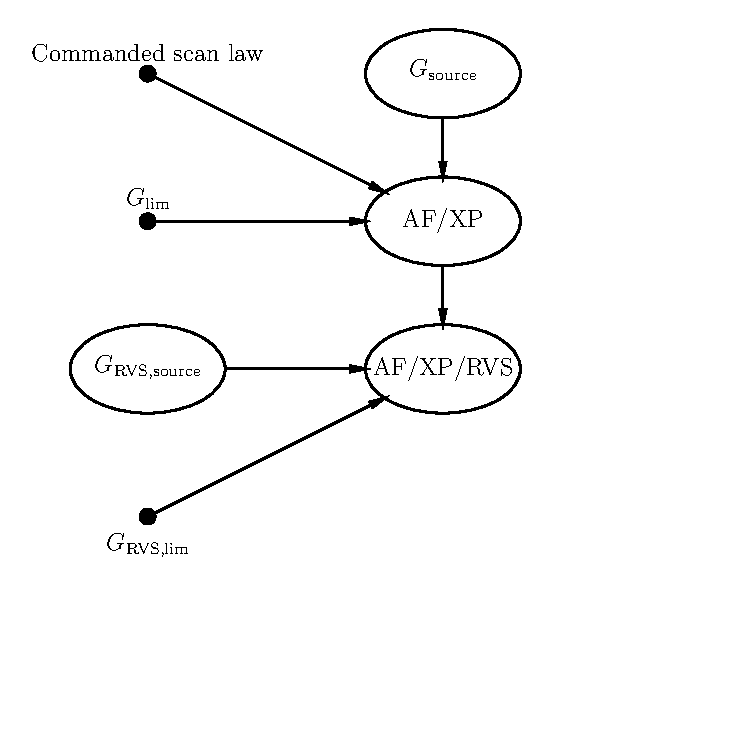
\includegraphics[height=8cm]{pgm_ideal_gsf.pdf}
    \caption{Idealized Gaia selection function. Here it is assumed that the spacecraft exactly follows the scan law as commanded from ground without any interruptions. The on-board decision on whether or not a source is observed depends only on the $G$ and $G_\mathrm{RVS}$ magnitudes of the source and the corresponding fixed survey limits. See text for a more detailed explanation.}
    \label{fig:gsf_ideal}
\end{figure}

\subsection{(b) Methodology}
\label{sec:methods}
\instructions{
    \begin{itemize}
        \item Describe and explain the overall methodology, distinguishing, as appropriate, activities
            indicated in the relevant section of the work programme, e.g. for research, demonstration,
            piloting, first market replication, etc.
    \end{itemize}
}

The Gaia selection function in an ideal world would look like the probabilistic graphical model shown in \figref{fig:gsf_ideal}. In this figure and the subsequent text the three main Gaia instruments as referred to as `AF' for Astrometric Field (collecting the astrometric data), `XP' which is short for the BP and RP photometric instruments, and RVS, the radial velocity spectrometer. The model in \figref{fig:gsf_ideal} shows that AF and XP observations of sources are collected whenever one of the Gaia telescopes scans over a source which has a magnitude $G_\mathrm{source}$ brighter than the magnitude limit $G_\mathrm{lim}$. If a source is bright enough in $G_\mathrm{RVS}$ data are also collected by the RVS instrument. The pointing of the Gaia telescopes is determined by a `scan law' which is fixed for the mission duration. The probability of a source entering the Gaia catalogue would thus be determined only by its true apparent magnitude $G_mathrm{source}$, the number of times the Gaia telescopes scanned across the source, and the uncertainty $\sigma_G$ in the on-board estimate of the source brightness. The probability that a radial velocity is listed in addition to astrometry and photometry would be determined independently by the true apparent magnitude of the source in the RVS wavelength range, $G_\mathrm{RVS,source}$, in combination with the scan law and the uncertainty $\sigma_{G_\mathrm{RVS}}$ of the on-board estimate of $G_\mathrm{RVS,source}$. The selection function for any derived data products, such as the astrophysical parameters of the sources, would be driven entirely by the basic data (astrometry, photometry, radial velocity, XP spectra, RVS spectra, or any combination thereof) used as inputs.

\begin{figure}[t]
    \centering
    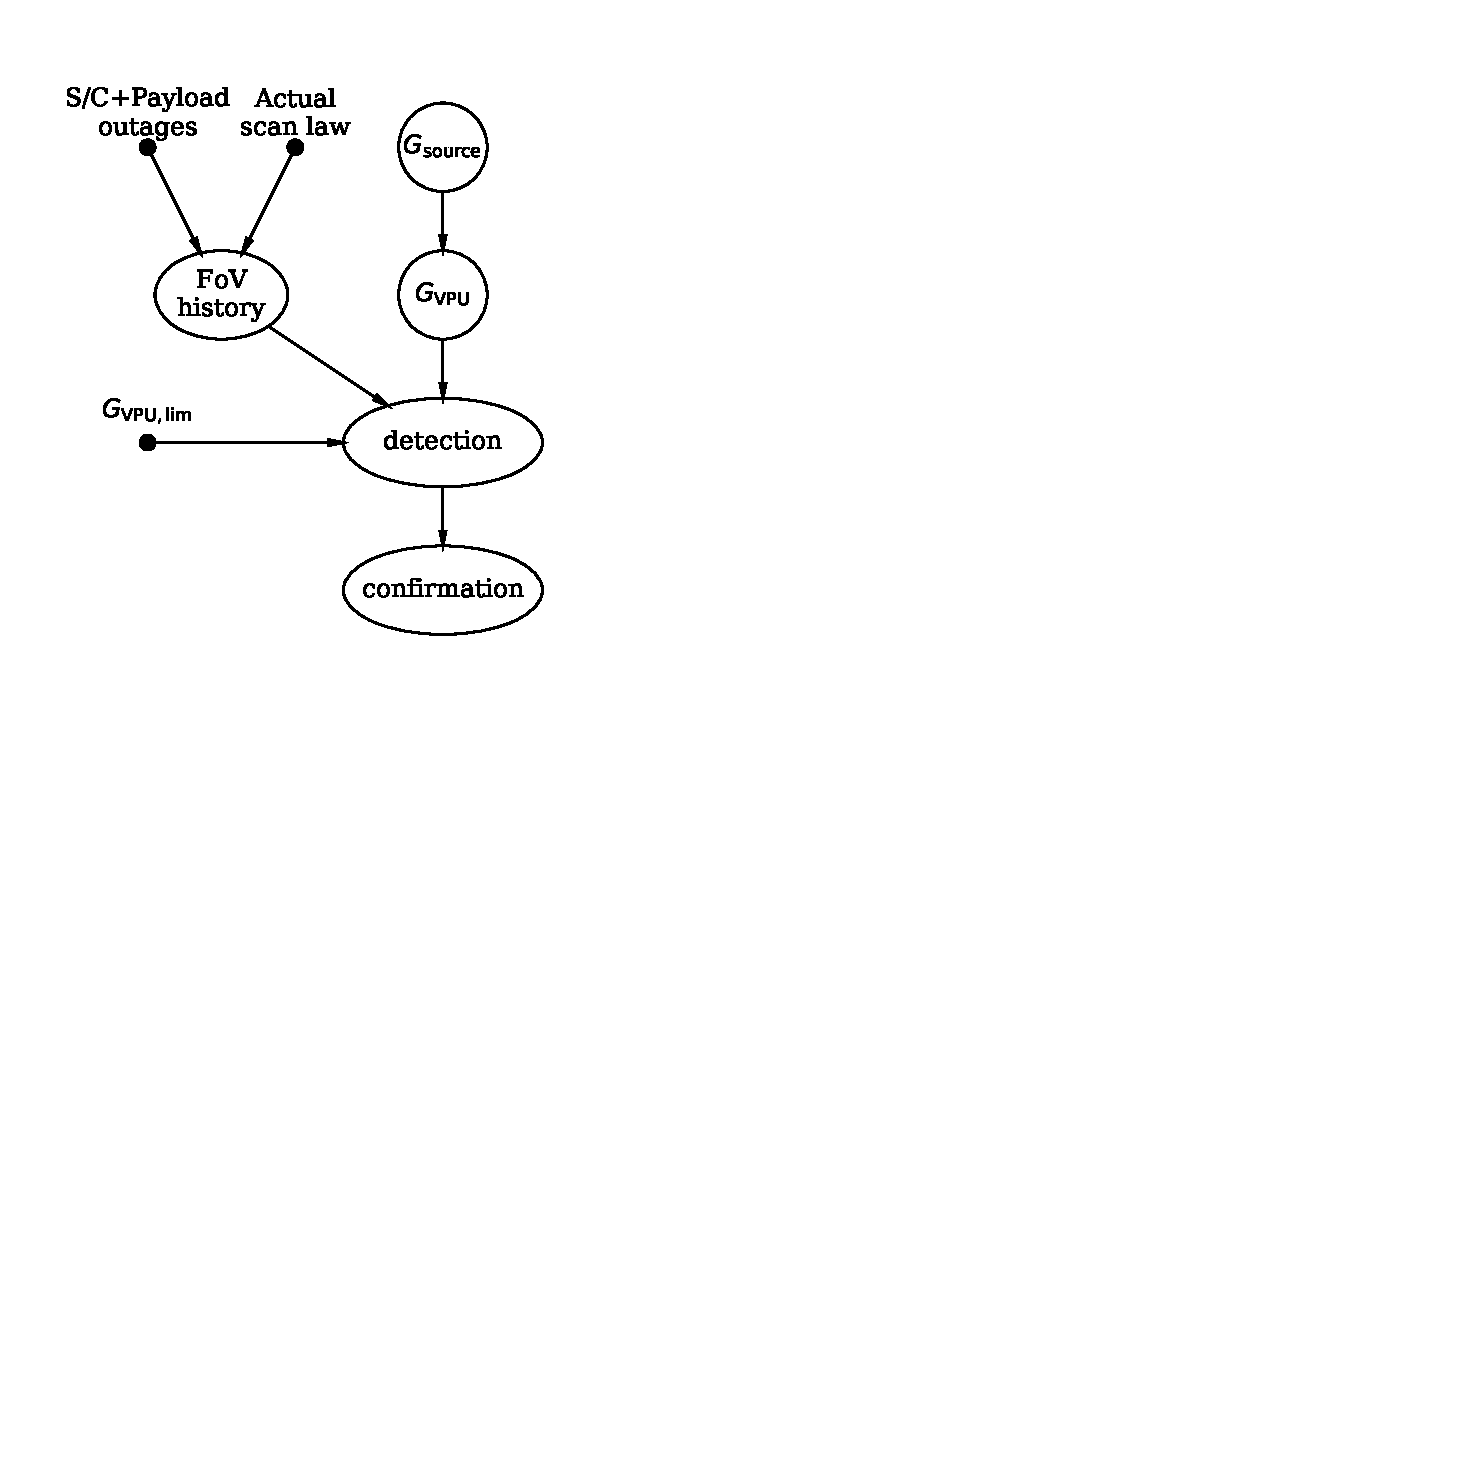
\includegraphics[width=\textwidth]{pgm_realistic_gsf.pdf}
    \caption{Simplified diagram of the actual Gaia selection function. The left hand side of the diagram provides a fairly complete picture of all the ingredients on-board the spacecraft that contribute to the selection function before the raw data is in hand on the ground. The right hand side shows in strongly simplified form how the Gaia selection function is further affected by the decision taken along the steps from the initial treatment of the raw data to the final published Gaia catalogue. See text for more detailed explanations.}
    \label{fig:gsf_realistic}
\end{figure}

In reality the Gaia survey selection function is vastly more complicated owing to the many stages in between source detection and final data product at which decisions are made on the spacecraft whether or not to make a certain observation, and in the on-ground data processing whether or not to include that observation. This is illustrated in \figref{fig:gsf_realistic}. The left hand side of the diagram shows the many decisions that are taken on-board the spacecraft which affect whether or not for a given source, passing through the field of view of one of the telescopes, measurements are actually collected.
\begin{itemize}
    \item The actual sky-scanning strategy executed by Gaia will differ from the desired one due to imperfections in the attitude control and interruptions of observations due to outages such as station keeping manoeuvres or on-board activities that require interrupting the measurement process (e.g., decontamination through heating of the payload, refocusing of the telescopes, more details can be found in \cite{2016A&A...595A...1G}).
    \item At the detection stage the brightness of the sources is estimated (with some uncertainty). This is indicated by $G_\mathrm{VPU}$ in the \figref{fig:gsf_realistic}, where VPU stands for `Video Processing Unit', essentially an on-board computer. In parallel an attempt is done to weed out spurious detections due to cosmic rays or PSF spikes, and sources are prioritized in order to deal with the limitation on the amount of sources that can be handled by the VPUs at any one time.
    \item Following confirmation that a detected source is real (through a second measurement of the source flux) astrometric and photometric data are collected, subject to further limitations in the amount of sources that can handled (indicated with 'VPU resource management' in \figref{fig:gsf_realistic}).
    \item RVS observations are collected only for sources bright enough in $G_\mathrm{RVS}$ which is estimated for bright sources through extrapolation from the on-board estimate $G_\mathrm{VPU}$ of $G_\mathrm{source}$ or through an estimate $G_\mathrm{RVS,VPU}$ from the flux in the RP spectrophotometric data. The latter introduces a source colour dependence.
    \item The data collected on-board is partly transmitted to the ground stations in real-time (during spacecraft contact periods) and is partly stored on-board for later transmission. The on-board storage limitations lead to data being deleted if it stays in the storage area too long (a consequence of limited availability of ground station time and the size of the data storage area). This happens primarily during so-called `galactic plane scans', when both Gaia telescopes are pointing at locations in the Milky Way plane on the sky. The data deletion decision is taken on the basis of a detailed priority table stored on-board. Additional data losses may occur due to lost telemetry packets (a minor contribution affecting roughly one in a million packets).
\end{itemize}

The left hand side of \figref{fig:gsf_realistic} shows a strongly simplified representation of further decisions taken along the DPAC pipelines on whether or not to process certain sources or parts of their data.
\begin{itemize}
    \item As a first step in the processing sources are classified as real or spurious, where the latter are typically caused by bright star PSF spikes or stray light features. Sources classified as spurious are `blacklisted' and subsequently not considered for processing. This classification process is imperfect.
    \item The next step is to group observations of the same source together and produce the so-called `source list'. This is a table linking a given source to all its observations. This process is redone from scratch for each data release and is subject to errors, such as observations being assigned to the wrong source, or the observations of one sources being assigned to multiple different sources. Two examples of specific challenges for the creation of the source list are crowded regions, where the source density on the sky can lead to observation to source matching uncertainties, and variable stars, where a strongly varying apparent brightness can confuse the matching process.
    \item Once the source list is created all subsequent processing steps are taken, from generating the astrometry, photometry, and radial velocity data, to the astrophysical characterization of sources, to the publication of a Gaia data release. At each step further decisions are taken on including or not sources or parts of their data. Often these decisions are explicitly or implicitly dependent on the source astrophysical parameters which will introduce further source brightness and colour dependencies into the selection function.
\end{itemize}

From the description above it is clear that the Gaia survey selection function is very complex and depending on the particular science case being addressed with Gaia data, the selection function must be known in great detail. An example is the list of binaries to be produced on the basis of Gaia data. The list will consist of various solution types (varying from mere indications of binarity to complete orbit solutions) which will be derived only for sources for which there is sufficient evidence that they are not single stars. The resulting list will thus be incomplete in a way that intricately depends on the binary star parameters, with many binaries still hiding among the sources not examined in detail in the DPAC pipeline.

The objective of this proposal is to derive a detailed description of the Gaia selection function which will be provided to and used by the scientific community. This will be done through the following tasks which map to the work packages listed in \secref{sec:work-plan} (the management task, work package \ref{wp:management}, is discussed in \secref{sec:management}).

\begin{description}
    \item[Operational definition of the Gaia survey selection function.] To guide the overall effort on the Gaia selection function it is important to precisely define what we mean by a selection function. We choose to take a probabilistic approach, thus asking the question: what is the probability of source X appearing in sub-sample Y of the Gaia catalogue? The mathematical formulation should at the top level be applicable to any astronomical survey but detailed mathematical definitions tailored to the Gaia survey may be needed. The formulation should account for the multiple layers of selection described above and allow for incomplete information on the data collection process. The formulation should also make it possible to accommodate additional user imposed selections (such as studying only sources with certain astrophysical parameters or demanding a minimum precision on the data used). A hierarchical probabilistic formulation is a natural choice but other approaches are not excluded. This task corresponds to work package \ref{wp:selfundefinition} and should be completed within the first 12 months of this project.
    \item[Specification of the Gaia selection function.] With the above mathematical formulation as the framework, this task is concerned with researching and working out in detail the description and modelling of the Gaia survey selection function (where we anticipate that some aspects cannot be described in all detail and will require simplifications or modelling). All the necessary information will be collected to describe or model in detail the elements in \figref{fig:gsf_realistic}, which will require close interactions with experts from the DPAC. An assessment will be made of the necessary level of detail to which the ingredients of the selection function must be known (in order to keep the scope of the effort realistic). The resulting description of the selection function will be hierarchical, starting from the basic selection steps and specializing to selection functions for specific subsets of the Gaia catalogue (such as, for example, the variable stars), and will allow for the inclusion of user imposed additional selection criteria. Part of this task will also be to collect data from other surveys which may aid in the understanding of the Gaia selection function. Examples are higher spatial resolution data from the Hubble Space Telescope to study selection effects in crowded regions, or photometric/spectroscopic data which can aid in the understanding of the selection effects on the distribution of source astrophysical parameters in Gaia samples. This task corresponds to work package \ref{wp:selfungaia}.
    \item[Tools to incorporate selection function in scientific analyses.] The aid the scientific community in using the Gaia selection function a set of data products and tools will be provided. The tools will implement in code the mathematical formulation and detailed description/modelling of the Gaia selection function. A means to layer user selections on top of the Gaia selection function will also be provided. The tools will be backed by the data products needed to use them such as numerical tables. These data products will be made available through, e.g., \url{https://zenodo.org/}, and in query-able form through the Gaia archive at ESA. The code underlying the tools will be open source and accessible through popular code-hosting facilities such as \url{https://github.com/}. Extensive documentation will also be provided in the form of papers in open access journals and detailed online documentation. This task corresponds to work package \ref{wp:selfunimplementation}.
    \item[Selection functions for combinations of Gaia and other surveys.] In many science applications the Gaia data will be combined with data from other surveys, often leading to the production of catalogues based on the input surveys \citep[see for example][]{2019A&A...628A..94A}. In such applications one needs to account for the combined selection function for the intersection of the surveys involved. In this task a generic method to combine survey selection functions will be researched and developed. The method will then be applied to generate selection functions for the combination of Gaia and a limited number of popular sky surveys. The tools and data products needed to combine selection functions will be made available through the channels mentioned above. The scientific community can use these to construct selection functions for other combinations of surveys. An important component of this task is making prototype versions of the tools publicly available and to bring users together in community workshop to use and test the tools. The feedback will be used to improve the prototypes. This task corresponds to work package \ref{wp:selfuncombine}.
    \item[Apply the selection function tools to selected science cases.] We believe that the best way to guide the overall efforts in this proposal and to thoroughly test the implementation of the Gaia survey selection functions, is to apply it to a number of science cases. The science cases will be developed in parallel to the selection function, both as a means to provide early tests of -- and feedback to -- the tasks above, and as a means to keep the researchers involved in this effort motivated. The results of the science applications will be published in the open access peer reviewed literature. It is very important for their future career that the post-doctoral researchers carrying out the bulk of the work will also have a publication featuring a science application to add to their CVs. This task corresponds to work package \ref{wp:scienceappl}.
\end{description}

\section{Ambition}
\label{sec:ambition}
\instructions{
    \begin{itemize}
        \item Describe the advance your proposal would provide beyond the state-of-the-art, and the
            extent the proposed work is ambitious.
        \item Describe the innovation potential (e.g. ground-breaking objectives, novel concepts and
            approaches, new products, services or business and organisational models) which the proposal
            represents. Where relevant, refer to products and services already available on the market.
            Please refer to the results of any patent search carried out.
    \end{itemize}
}

As pointed out in \secref{sec:objectives} there is currently no detailed selection function available for the Gaia survey. It is not part of the DPAC tasks or data products, and the limited attempts that have been made in the community to characterize the selection function have led mostly to ad-hoc implementations for specific science cases. In fact the vast majority of works on the Gaia data so far ignore the selection effects altogether. More generic attempts at describing the Gaia selection function have been undertaken by Boubert \& Everall\footnote{\url{https://github.com/DouglasBoubert/selectionfunctions}}, and by Rybizki, Drimmel \& Carrasco\footnote{\url{https://github.com/jan-rybizki/gdr2_completeness}}. However, these efforts only scratch the surface of the complexities of the Gaia selection function. The efforts proposed here will thus go well beyond the state of the art:
\begin{itemize}
    \item For the first time a Gaia survey selection function will be provided at the level of detail and with the tools needed to take it into account in any science application.
    \item The efforts to describe and implement the Gaia selection function will lead to a clarification and better definition of the concept of selection functions and biases. This will benefit the development of selection functions for other surveys.
    \item The availability of the selection function will enhance all the scientific analyses of the Gaia data. This will lead to a much better scientific exploitation of the Gaia data in that selection biases can be properly accounted for, while the availability of open source tools and corresponding open access data will facilitate a much better reproducibility of results.
    \item The innovations in terms of the mathematical formulation of the selection function and a usable detailed practical implementation thereof can be transferred to other sky surveys, both past and future, enhancing the quality of the scientific exploitation and their legacy value.
\end{itemize}

%%% Local Variables:
%%% mode: latex
%%% TeX-master: "proposal-main"
%%% End:
